\section{Introduction}
Bien que dans les chapitres précédents nous avons vu qu'il était possible d'estimer de
façon fiable la contribution des différentes sources de PM grâce aux PMF et d'étblir une
phénoménologie des sources de \PMdix, la question de leur effet sanitaire n'est toujours
pas répondu. En effet, l'ordre de contribution à la concentration moyenne anuelle des
\PMdix{} présenté par \cite[(figure 3)]{weberComparison2019} ne préjusage pas de leur impacte
sanitaire.

En effet, comme détaillé dans en introduction
section~\ref{sec:le_potentiel_oxydant_des_aerosols}, la mesure de la masse des PM n'est
certainement pas l'indicateur le plus adapté pour évaluer leur toxicité car la composition
chimique, forme, surface réactive, etc. n'est pas prise en compte par cette métrique.
C'est pourquoi le potentiel oxydant (PO ou OP en anglais), mesurant indirectement les
espèces réactives de l'oxygène (ERO ou ROS en anglais) apportées ou induites par les PM,
est proposé comme nouvel indicateur de l'exposition des populations à la toxicité des PM. 
Il est maintenant bien documenté que les différents tests de PO présentent une information
différente de la concentration massique (voir par exemple,
\cite{choRedox2005,vermaReactive2014,batesReactive2015,fangOxidative2016,fangAmbient2017,calasSeasonal2019},
ou la revue détaillée récente de \cite{batesReview2019}), comme rappelé dans le
tableau~\ref{tab:calas_2018_spearman} sur une étude à Chamonix par
\cite{calasComparison2018} présentant la corrélation entre la masse des \PMdix{} et 5
mesures de PO.

Il est également connu que les différentes espèces chimiques constitutives des PM ne
réagissent pas à un même test de PO de la même manière. Notamment, les métaux de
transitions  ainsi que certaines quinones conduisent à la formation d'un grand nombre de
\ce{HO^.} et sont donc des espèces très réactives à la mesure du PO
\autocite{charrierRates2015,calasImportance2017}.

Cependant, lorsque l'ensemble des PM est solubilisé, analysé et confronté aux PO, de
fortes corrélations sont bien observés avec les espèces présentant un forte réactivité aux
PO, mais certaines autres espèces sont parfois fortement corrélé alors qu'une mesure
directe du PO du nitrate ne montre aucune réactivité --c'est notamment le cas du nitrate,
de l'ammonium ou de lévoglucosan \autocite{vermaRedox2009,calasComparison2018,calasSeasonal2019}.

Ces corrélations ne reflètes donc pas de réelles causalité mais des co-corrélations. Le
lévoglucosan est émis en même temps que certaines quinones lors de la combustion de bois,
qui elles sont redox-active, et le nitrate est émis temporellement en fin d'hiver-début
printemps, où la combustion de biomasse est toujours présente. 
Ainsi, ces corrélations sont un premier pas vers l'identification des sources majoritaires
de PO, mais s'avère insuffisant.

Je propose dans ce chapitre d'utiliser la méthode suivante, résumé dans la
figure~\ref{fig:workflow_inversion} pour estimer les sources de potentiel oxydant :
\begin{enumerate}
    \item Estimer les sources de PM grâce à la chimie et une étude PMF;
    \item Utiliser un modèle de régression linéaire multiple entre les sources issus
        des PMF et les PO;
\end{enumerate}

\begin{table}[ht]
    \begin{ThreePartTable}
        \centering
        \caption{Corrélation de spearman entre 5 tests de PO et la masse des \PMdix{} sur
            le site de Chamonix (2013) séparer en période chaude (triangle bas) et froide
            (triangle haut).\\
            Source : \cite[Table 3]{calasComparison2018}
        }
        \label{tab:calas_2018_spearman}
        \footnotesize
        \begin{tabular}{lSSSSSS}
            \toprule
             & {\PMdix} & {OP DTTv\tnote{1}} & {OP AAv\tnote{1}} & {OP ESRv\tnote{2}} & {OP GSHv\tnote{1}} & {OP ASCv\tnote{3}}\\
             \midrule
            \PMdix  &           & 0.91{***} & 0.91{***} & 0.59{***} & 0.87{***} & 0.90{***}\\
            OP DTTv & 0.71{***} &           & 0.89{***} & 0.61{***} & 0.79{***} & 0.72{***}\\
            OP AAv  & 0.43{*}   & 0.65{***} &           & 0.54{***} & 0.85{***} & 0.79{***}\\
            OP ESRv & 0.088     & 0.17      & 0.36      &           & 0.56{**}  & 0.59{**}\\
            OP GSHv & 0.44{*}   & 0.29      & 0.36      & 0.63{*}   &           & 0.92{***}\\
            OP ASCv & 0.38{*}   & 0.37{*}   & -0.072    & -0.29     & 0.17      & \\
            \bottomrule
        \end{tabular}
        \begin{tablenotes}
        \item[] *** p < 0.001 level, ** p < 0.01 level, * p < 0.05 level
        \item[1] n = 30 (cold period), n = 29 (warm period)
        \item[2] n = 30 (cold period), n = 14 (warm period)
        \item[3] n = 27 (cold period), n = 29 (warm period)
        \end{tablenotes}
    \end{ThreePartTable}
\end{table}

\begin{figure}[ht]
    \centering
    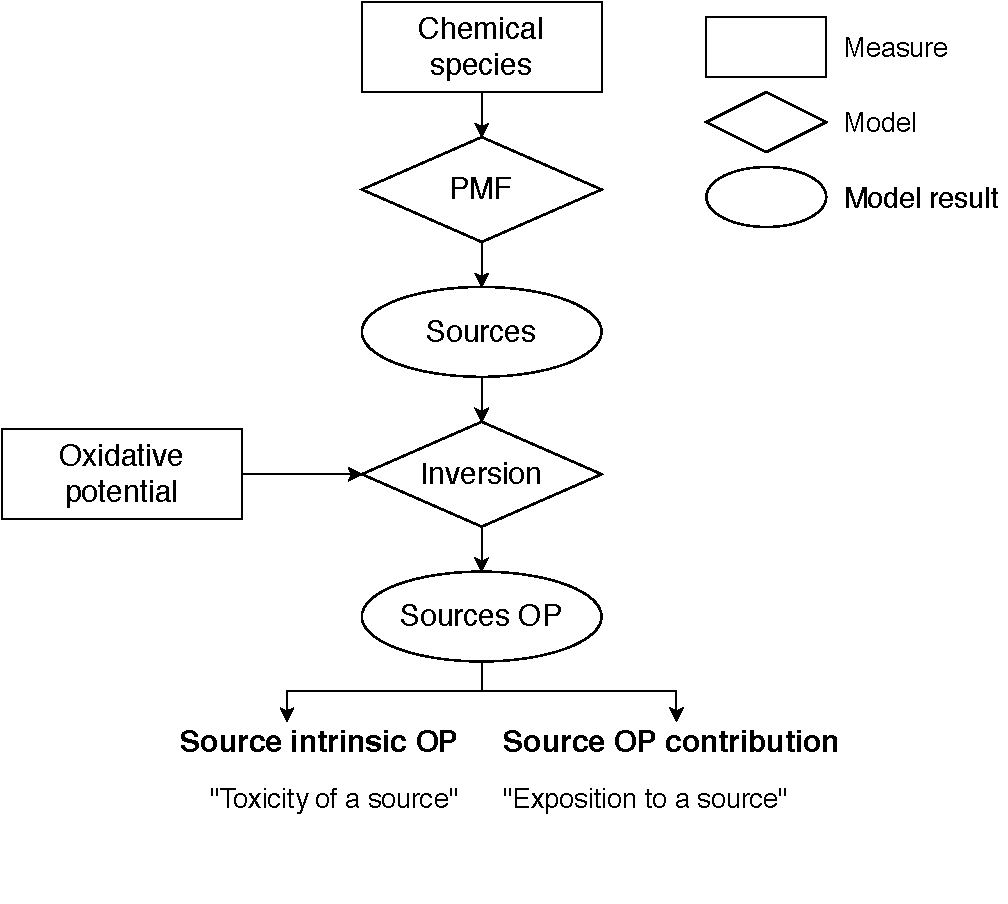
\includegraphics[width=0.8\linewidth]{figures/chapter04/flowchart_inversion.pdf}
    \caption{Processus suivi afin d'estimer la contribution des sources de PM aux
        potentiels oxydants. La méthode d'inversion utilisée dans ce chapitre est une
        régréssion linéaire multiple, permettant d'attribuer un PO par microgramme de source
        (\textit{PO intrinsèque}), estimant la ``toxicité de la source'', et la contribution de
    chacune des sources aux PO, estimant l'exposition de la population à cette source.}%
    \label{fig:workflow_inversion}
\end{figure}

\section{Dévelopemment méthodologique à Chamonix}%
\label{sec:dévelopemment_méthodologique_à_chamonix}

\clearpage
\section{Apportionment method for the oxidative potential of \PMdix{}}
\label{sec:weber_et_al_2018}

Article paru dans le journal \textit{Atmospheric Chemistry and Physics} le 4 juin 2019 :

\begin{quote}
    Samuël Weber, Gaëlle Uzu, Aude Calas, Florie Chevrier, Jean-Luc Besombes,
    Aurélie Charron, Dalia Salameh, Irena Ježek, Griša Močnik, et Jean-Luc Jaffrezo. 2018.
    \textit{An Apportionment Method for the Oxidative Potential of Atmospheric Particulate
    Matter Sources: Application to a One-Year Study in Chamonix, France}. Atmospheric
    Chemistry and Physics 18(13), pp. 9617‑9629.
    \textsc{doi} : \href{https://doi.org/10.5194/acp-18-9617-2018}{10.5194/acp-18-9617-2018},
    \textsc{url} : \url{https://www.atmos-chem-phys.net/18/9617/2018/}
\end{quote}

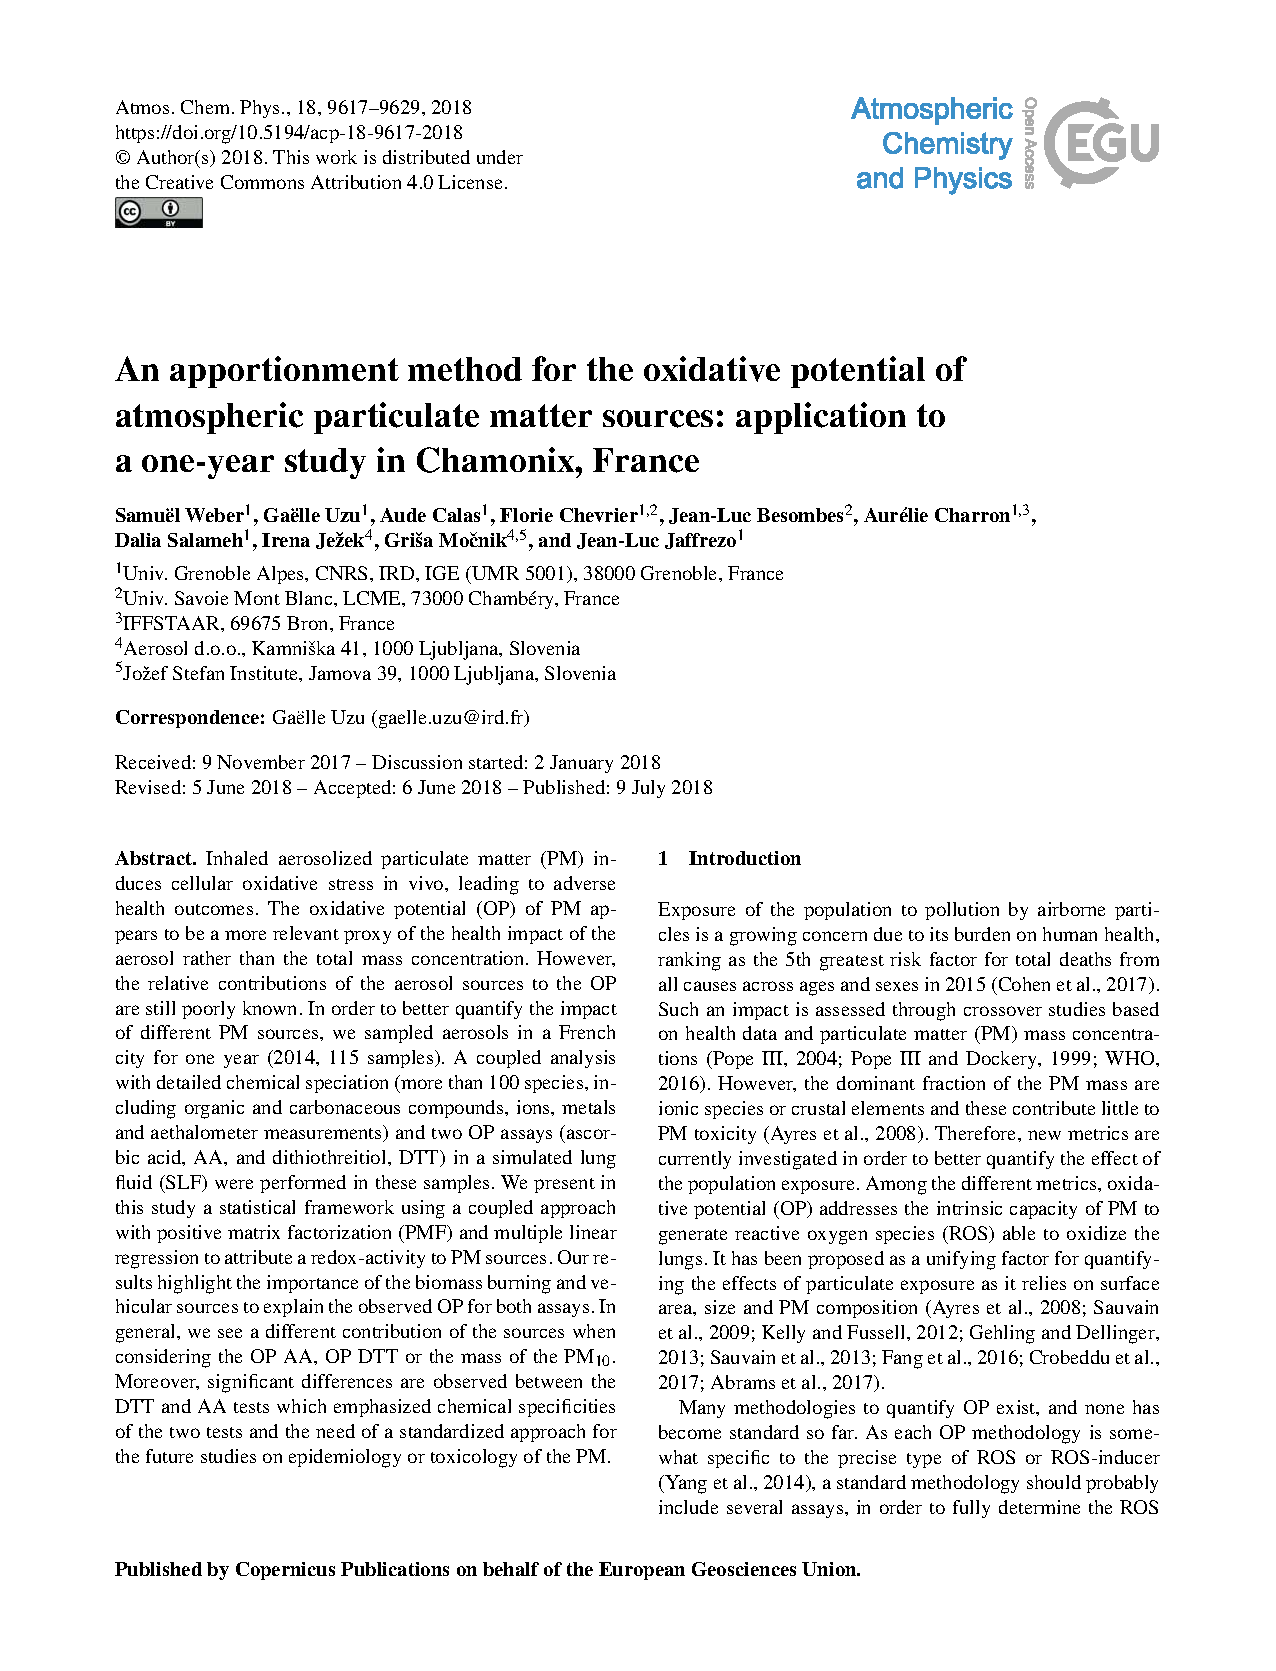
\includepdf[pages=-,scale=0.95,pagecommand={\pagestyle{fancy}}]{chapters/deconvol_OP.pdf}


\section{Conclusion}
